%!TeX spellcheck = en_GB
\documentclass[conference]{IEEEtran}
\IEEEoverridecommandlockouts
\usepackage{cite}
\usepackage{amsmath,amssymb,amsfonts}
\usepackage{algorithmic}
\usepackage{graphicx}
\usepackage{textcomp}
\usepackage{xcolor}

\begin{document}
    
    % describe the protocol for control access (blockchain part)
    %  Related work
    %    -   traditional architectures commonly employed in the IoT access:
    %       XACML, OAuth, UMA
    %       Dependency of a central entity

%\title{Fine-grained Authorized Medical Data Management}
\title{Blockchain-based Bidirectional Updates on Fine-grained Medical Data}
%\title{Distributed Authorized Medical Data Management}
%\title{Distributed Authorized Medical Data Updates}
%\title{Authorized Updates to Distributed Medical Data}

% We talk more about updates, shall we just use updates on the title?

\author{
    \IEEEauthorblockN{%
        Chunmiao Li\textsuperscript{1,3},
        Yang Cao\textsuperscript{2},
        Zhenjiang Hu\textsuperscript{1,3,4},
        Masatoshi Yoshikawa\textsuperscript{2}
    \vspace{1.5ex}
    \IEEEauthorblockA{%
        \textsuperscript{1}\,National Institute of Informatics, Japan\qquad
        \textsuperscript{2}\,Kyoto University, Japan \\
        \textsuperscript{3}\,SOKENDAI (The Graduate University for Advanced Studies), Japan\qquad
        \textsuperscript{4}\,University of Tokyo, Japan
    }
%    \vspace{1ex}
%    \IEEEauthorblockA{%
%        Email:\
%        \textsuperscript{1}\,chunmiaoli1993@nii.ac.jp,
%        \textsuperscript{2}\,yang@i.kyoto-u.ac.jp,
%        \textsuperscript{3}\,hu@nii.ac.jp,
%        \textsuperscript{4}\,yoshikawa@i.kyoto-u.ac.jp
%    }
}
}

\maketitle

%regulate the use of a, an, the
\begin{abstract}
    Electronic Medical data sharing between stakeholders, such as patients, doctors, and researchers, can promote more effective medical treatment collaboratively. These sensitive and private data could only be accessed by authorized users.  Given a total medical data, users may care parts of them and other unrelated information might interfere with the user-interested data search and increase the risk of exposure. Besides accessing these data, users may want to update them and propagate to other sharing peers so that all peers keep identical data after each update. To satisfy these requirements, in this paper we propose a medical data sharing architecture that addresses the permission control using smart contracts on blockchain and splits data into fined-grained pieces shared with different peers then synchronize complete data and these pieces with bidirectional transformations. Medical data reside on each user's local database and permission-related data are stored on smart contracts. Only all peers have gained the newest shared data after updates can they start to do next operations on it, which are enforced by smart contracts. Blockchain-based immutable shared ledge enables users to trace data updates history. This paper can provide a new perspective to view complete medical data as different slices to be shared with various peers but consistency after updates between them are still promised, which can protect privacy and improve data search efficiency.

\end{abstract}

\begin{IEEEkeywords}
medical data, blockchain, update, bidirectional transformations
\end{IEEEkeywords}

\section{Introduction}

Now a lot of medical data are digitalized so as to be stored and accessed conveniently. A medical record is produced after a patient goes to see a doctor and often resides on the hospital's database. Medical records usually contain highly sensitive information about patient privacy. HIPPA Privacy Rule  \cite{centers2004hipaa} in the U.S. regulates the use and disclosure of personally identifiable health information to protect patients' privacy. However, it hard to make sure that all medical institutes would follow these rules and they may expose patient privacy for profit. Moreover, patients might visit many hospitals and leave their records scattered \cite{zhang2016secure} in different places, so that it is hard for them to manage records efficiently. Patients should better to be provided a platform to manage and review their historical medical data in case of exposure or being tampered. What's more, better communication between patients and doctors can contribute to patient adherence \cite{zolnierek2009physician} and improve health \cite{street2009does}. In addition to provide data to doctors, patients tend to share their medical data with health experts to help understand some complex statistics. Many kinds of research have been done to study how medical specialists with different expertise collaborate with each other \cite{fitzpatrick2013review}.  Researchers can identify public health risks and then develop a better treatment by analyzing existing medical data \cite{office2015report}. 
%As presented in \cite{chung2018using},  patients and experts can exchange information to develop better plans to satisfy individual routines. 
Sharing medical data under some constraints could benefit all relating stakeholders such as patients, researchers, and doctors. 
% %patient understand and trace his medical records
% %doctor revise treatment plan in terms of feedback
% %researcher conduct census analyzation and provide better measures

To protect patients' data from being exposed or tampered, shared medical data could reside in encrypted formats on a trusted cloud storage server and can only be accessed by authorized users. However, in that case, centralized access control might lead to a single point of failure and become the bottleneck of the sharing system. Some decentralized medical data sharing systems \cite{azaria2016medrec,fan2018medblock,xia2017bbds} have been proposed to manage authentication based on blockchain\cite{nakamoto2008bitcoin} technology, which achieves consensus among distributed nodes. The access control logic of medical data is encoded into smart contracts\cite{azaria2016medrec} or Chaincode \cite{dubovitskaya2017secure} so that anyone who wants to access medical data should firstly be authorized permission from the blockchain side.

% and their access process will be recorded on the blockchain.

Still, we identified a limitation on current works. Users might be overwhelmed by a complete medical record since they tend to have a unique focus on it. For example, given a medical record, researchers are interested in the mechanism of medicine action, whereas patients care more about the medicine dosage standard.  In addition, additional but unnecessary information might influence or even mislead users' judgment. Imagine that doctors may add some symptom description on records which might put patients in confusion and fear \cite{delbanco2010open}. In addition, treatment steps are exclusive to a hospital and can not be directly accessed to other users.

To fill this gap, we propose an idea that a complete medical data (i.e., data source) might be split into lots of smaller pieces (i.e., data views). A user can share different fine-grained data pieces\footnote{Our work assume that the initialization of shared data has been finished. We only consider management on existing shared data.}  with different users based on predefined protocols. Imagine a doctor can share dosage usage with a patient and medicine mechanism with a researcher respectively. In this way, only users related data are exposed to them, which can avoid additional data interference and protect private data from being leaked. 

However, if we adopt this idea, we have to dispose of the synchronization between source and multiple views when updates on shared data occur. Consider this scenario: a researcher updates the medicine mechanism on shared data with a doctor. Note here the shared data is actually a view from the complete medical data (source) on the doctor side. Thus he needs to synchronize this change on view to create a new source. 

%Current works mostly only consider uni-directional updates on shared data, which means that these updates are conducted by data providers and then produce modified data to other users. They did not offer the synchronization scheme between source and views on the same user side.

To solve this problem, we apply bidirectional transformations \cite{hu2014validity} to synchronize them after updates on either one side. For example, we can invoke \emph{put} direction of a  BX program to reflect modifications on shared data in complete data and \emph{get} to produce shared data from complete data. Because different views produced from the same source might have overlapped data. The doctor still has to judge whether he needs to modify the shared data with patients by reproducing a new view.


%read, add, delete shared data belong to data management.
%Since the shared data just reside in each peer's local database, read the shared data is easily promised.

%For authorization
Moreover,  we encode permission information of shared data into smart contracts. Shared data management should be conducted after the peer has been authorized. 

%Any modifications on the existing shared data should be updated to all sharing peers immediately. 

%We store the sharing peers' identity not pointers to the raw data into smart contracts in case of private data leakage. 

%Each sharing peer will receive the notification from smart contracts after updates on shared data are verified. Then each peer will request the newest data from updater and then use it to update his local complete data. Smart contracts will refuse any further operations on shared data before all sharing peers have pulled the newest data to their local database.

In this paper, our contributions are as follow.
\begin{enumerate}

    \item We proposed to partition a complete medical record to multiple more fine-grained data pieces shared with different peers and apply bidirectional transformations to synchronize a record and these multiple pieces.
    
    \item We designed a decentralized medical data sharing architecture where data reside on user's local database and metadata are stored on smart contracts of blockchain to control permission for managing data.
        
    \item We sketched procedures for data management (i.e., Create, Read, Update, Delete) operations on shared data.
    
%    \item We surveyed existing blockchain-based medical data sharing solutions and clarified their disadvantages, which are presented in Section \ref{related work};

\end{enumerate}

The remainder is organized like this. Section \ref{preli} gives some preliminaries about blockchain and bidirectional transformations. Section \ref{system} sketches our system design and provides an implementation architecture. Section \ref{threats} discusses identified threats and proposes countermeasures. Section \ref{related work} compares our work with existing ones to clarify our improvement over them. Section \ref{conclude} concludes and directs our future work.

\section{Preliminaries}
\label{preli}

    \subsection{Blockchain}
    Proposed with Bitcoin \cite{nakamoto2008bitcoin} in 2008, blockchain technology has been widely used in many fields. Blockchain provides a solution for data storage, data transfer and consensus protocol in a distributed and decentralized environment. Generally speaking, blockchain is a shared ledger and replicated by all nodes on a distributed network, which records the historical valid transactions in chronologically chained blocks. The nodes who generate new blocks by solving a computational puzzle (the proof-of-work problem) are called miners.
    
    Not only can support the platform of cryptocurrency, but blockchain can also be applied to other scenes. Ethereum \cite{wood2014ethereum} extend blockchain with additions such as a built-in Turing-complete programming language so that one can use this scripts (i.e., Ethereum Virtual Machine (EVM) bytecodes) to write programs (i.e., smart contracts\footnote{Hyperledger and others still provide platforms to write smart contracts.}) on the blockchain. We can just write Solidity\footnote{https://solidity.readthedocs.io/en/v0.5.2/} programs and then compile it to EVM code. Besides the user accounts controlled by private keys like in Bitcoin, the accounts for smart contracts are allowed in Ethereum. Anyone can build decentralized applications which consist of a collection of smart contracts. Once a transaction involving smart contract creation gets confirmed, an address is generated for the contract and later anyone can send transactions to this address to execute the programs on it. A smart contract transaction is enforced when a miner includes it in a new produced block. Other nodes will validate it and re-run contracts if it is valid.
    
    \subsection{Bidirectional transformations}
    %Two directions are good, but hard to keep well behaveness. Once change one side, need to modify another side.
    % BXs: write one program to express two directions 
    % get-based may relate to multiple puts for one get
    % put-based is injective and better 
    Maintaining consistency between different data representations having overlapping contents is important \cite{abou2018introduction}. For example, in databases, a view table can be produced by querying a base source table; this view table can be modified, in which case we will want to ``restore consistency", i.e.,  we need to change the source such that the modified view coincides with the result of the query on the changed source --- this is the well-known view update problem \cite{bancilhon1981update}. To achieve this, one may consider providing two separate programs to represent the two directions to propagate updates from one side to the other. But it is hard to prove that the source and view can still be kept consistent after updates. Bidirectional transformations (BXs) were proposed  \cite{czarnecki2009bidirectional} to solve this.
    
    BX programs\footnote{The BXs we refer to in this paper are asymmetric lenses \cite{foster2007combinators}, one of the synchronization models studied by the BX community. } can be invoked in two ways as forward and backward transformations. A forward transformation (denoted as \emph{get}) extracts some information from the source to build an abstract view, and the backward transformation (denoted as \emph{put}\footnote{\emph{put} is not a simple inverse of \emph{get}. Instead, it accepts the view and the original source as input and produces an updated source as output.}) embeds information of the view back into the source and produces an updated source. This pair of transformations should satisfy the {\em round-tripping} laws (also referred to as {\em well-behaveness}) called \emph{PutGet} and \emph{GetPut}. 
    \begin{align}
    get (put(\textbf{source}, \textbf{view}))= \textbf{view} \tag {\emph{PutGet}} \\
    put (\textbf{source}, get (\textbf{source})) = \textbf{source} \tag {\emph{GetPut}} 
    \end{align}
    
    Intuitively, \emph{GetPut} states that no update should be performed on the source when there is no change on the view, while \emph{PutGet} hints that \emph{put} should take all updates on the view into account so that the view can be regenerated from the updated source by \emph{get}. 
    The most distinguished point of BX is that a view can contain only a part of a source. With respect to some consistency between a source and a view, BX programs can synchronize the source and view, and their well-behavedness guarantees that the source and view are kept consistent after updates on either side. There are some languages for constructing well-behaved BX programs, such as Boomerang\cite{bohannon2008boomerang}, BiGUL \cite{bigul} and HOBiT\cite{matsuda2018hobit}.
    
%    One BX program can represent the two transformations and we can achieve the transformation from one side to the other by invoking the  \emph{get} or \emph{put} direction of the program. 

    %which has been developed for putback-based bidirectional programming.

\section{System architecture}
\label{system}

In this section, we first present the way to split a complete medical record into multiple pieces in Section \ref{fine-grained}. Then Section \ref{permission} shows the permission encoding on smart contracts. Our system can not only allow updates on shared data but other operations such as creating data, which are described in Section \ref{dataManage} and explained by a concrete case in Section \ref{updateCase}. Lastly, we give our system architecture on Section \ref{architecture}.
     
%     Part A describes the data\footnote{In our prototype, medical data are entered directly by users. Later we may consider using the data from wearable devices.} distribution between sharing peers. Part B explains our system architecture.
To simplify our expression next, we adopt nodes and users to denote devices connecting to blockchain network and stakeholders (doctors, patients, etc.) in medical scenarios respectively. Users sharing data are called sharing peers.
     
%\subsection{Data distribution}
\subsection{Fine-grained shared data}
\label{fine-grained}

% If we build a big contract which is a list of list and each small list is a contract for a shared data

Shared data\footnote{In our prototype, medical data are entered directly by users. Later we may consider using the data from wearable devices.} can exist in different peers, as shown in Fig. \ref{workflow}.  Suppose there are three users: patient Alice, researcher Charlie, and doctor Bob. Each user has their own complete base table which is named as D1, D2, D3 respectively and different shared data with other users. For example, Bob and Charlie share some data which are stored in D32 on Bob side and D23 on Charlie side respectively. D32 and D23 should contain the same contents, which means either one is updated and the other one need be modified to become identical with it again. Similarly, Alice and Bob share the same contents that stored in D13 and D31 separately in their sides. Notably, the formats and contents of shared data are predefined by sharing peers. 

\begin{figure}[htbp]
    \centerline{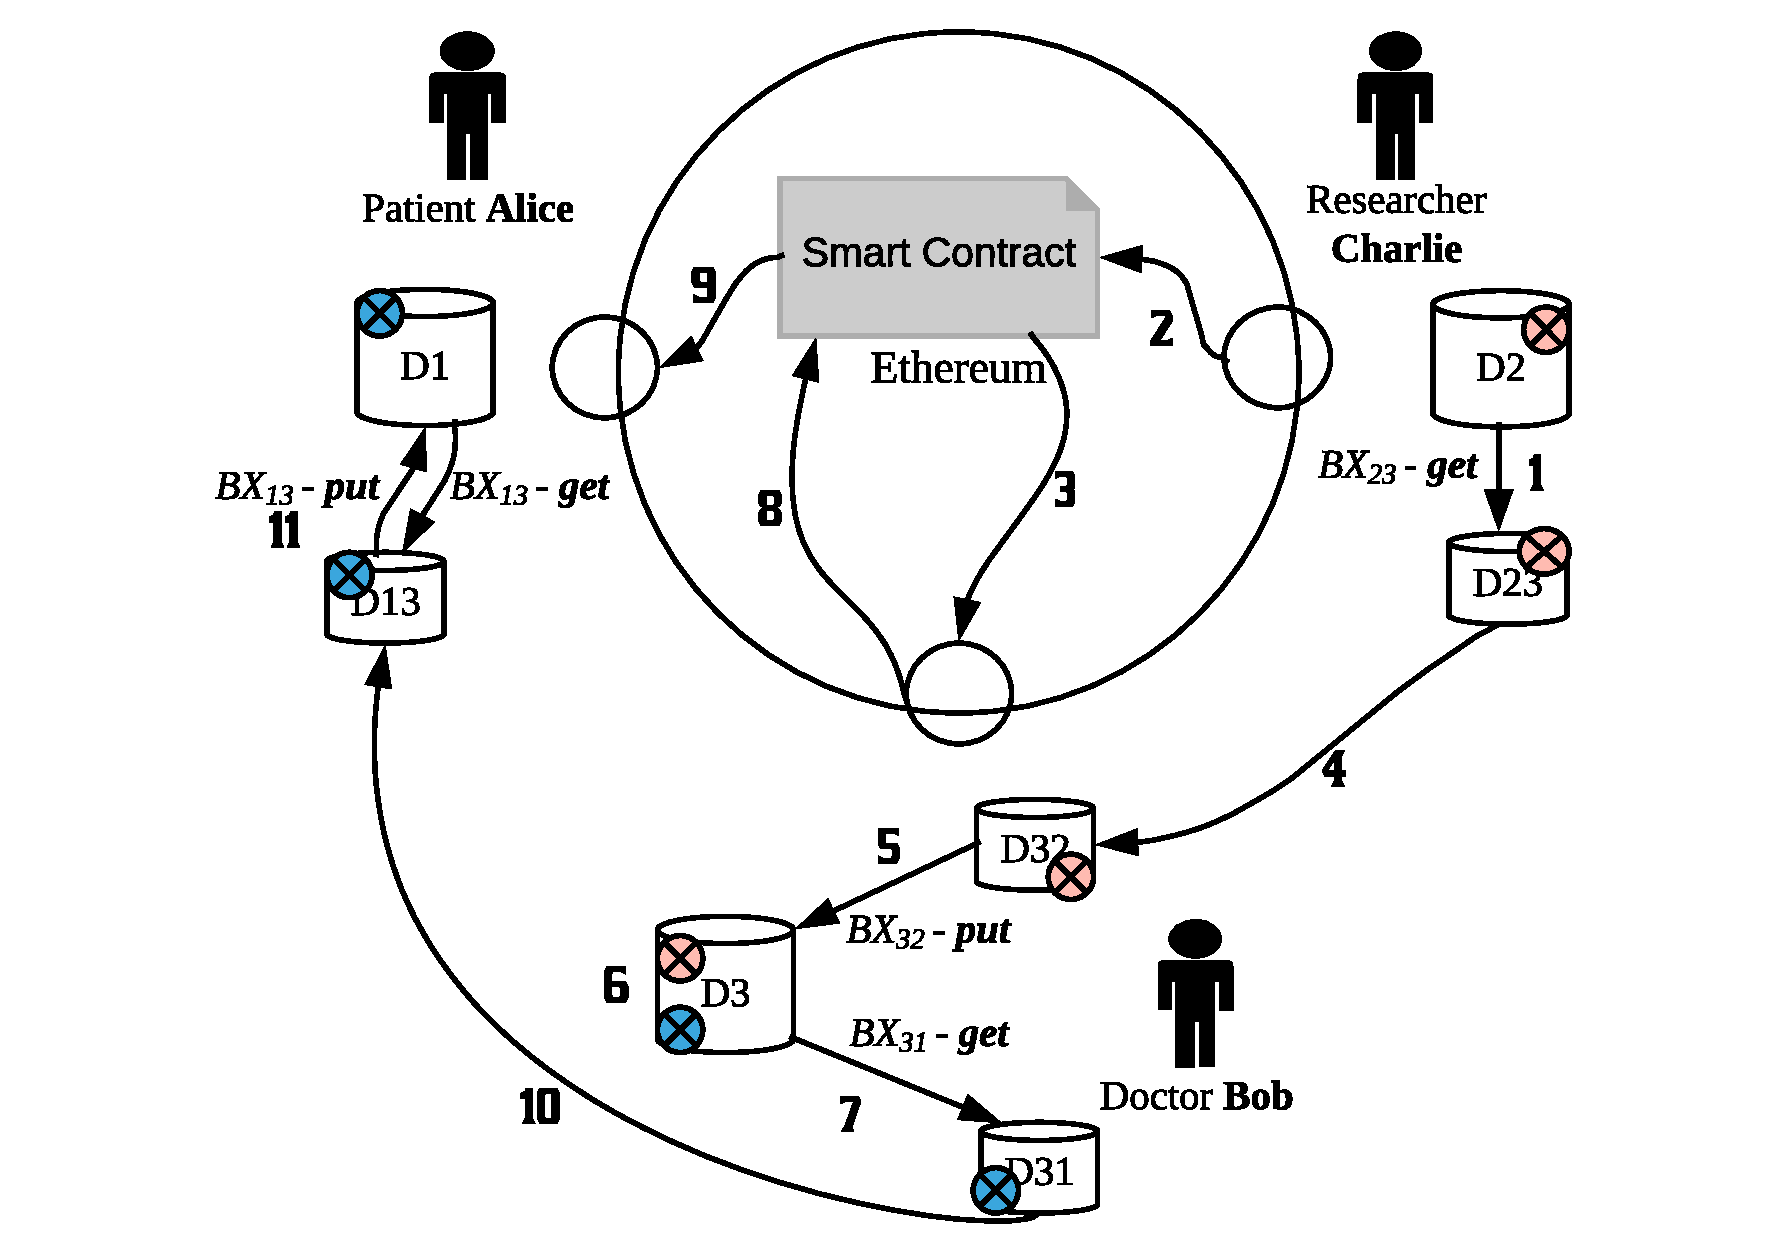
\includegraphics[width=270pt,height=220pt]{updateScenario.pdf}}
    \caption{A workflow for updating data fields of shared data}
    \label{workflow}
\end{figure}

\begin{figure}[htbp]
    \centerline{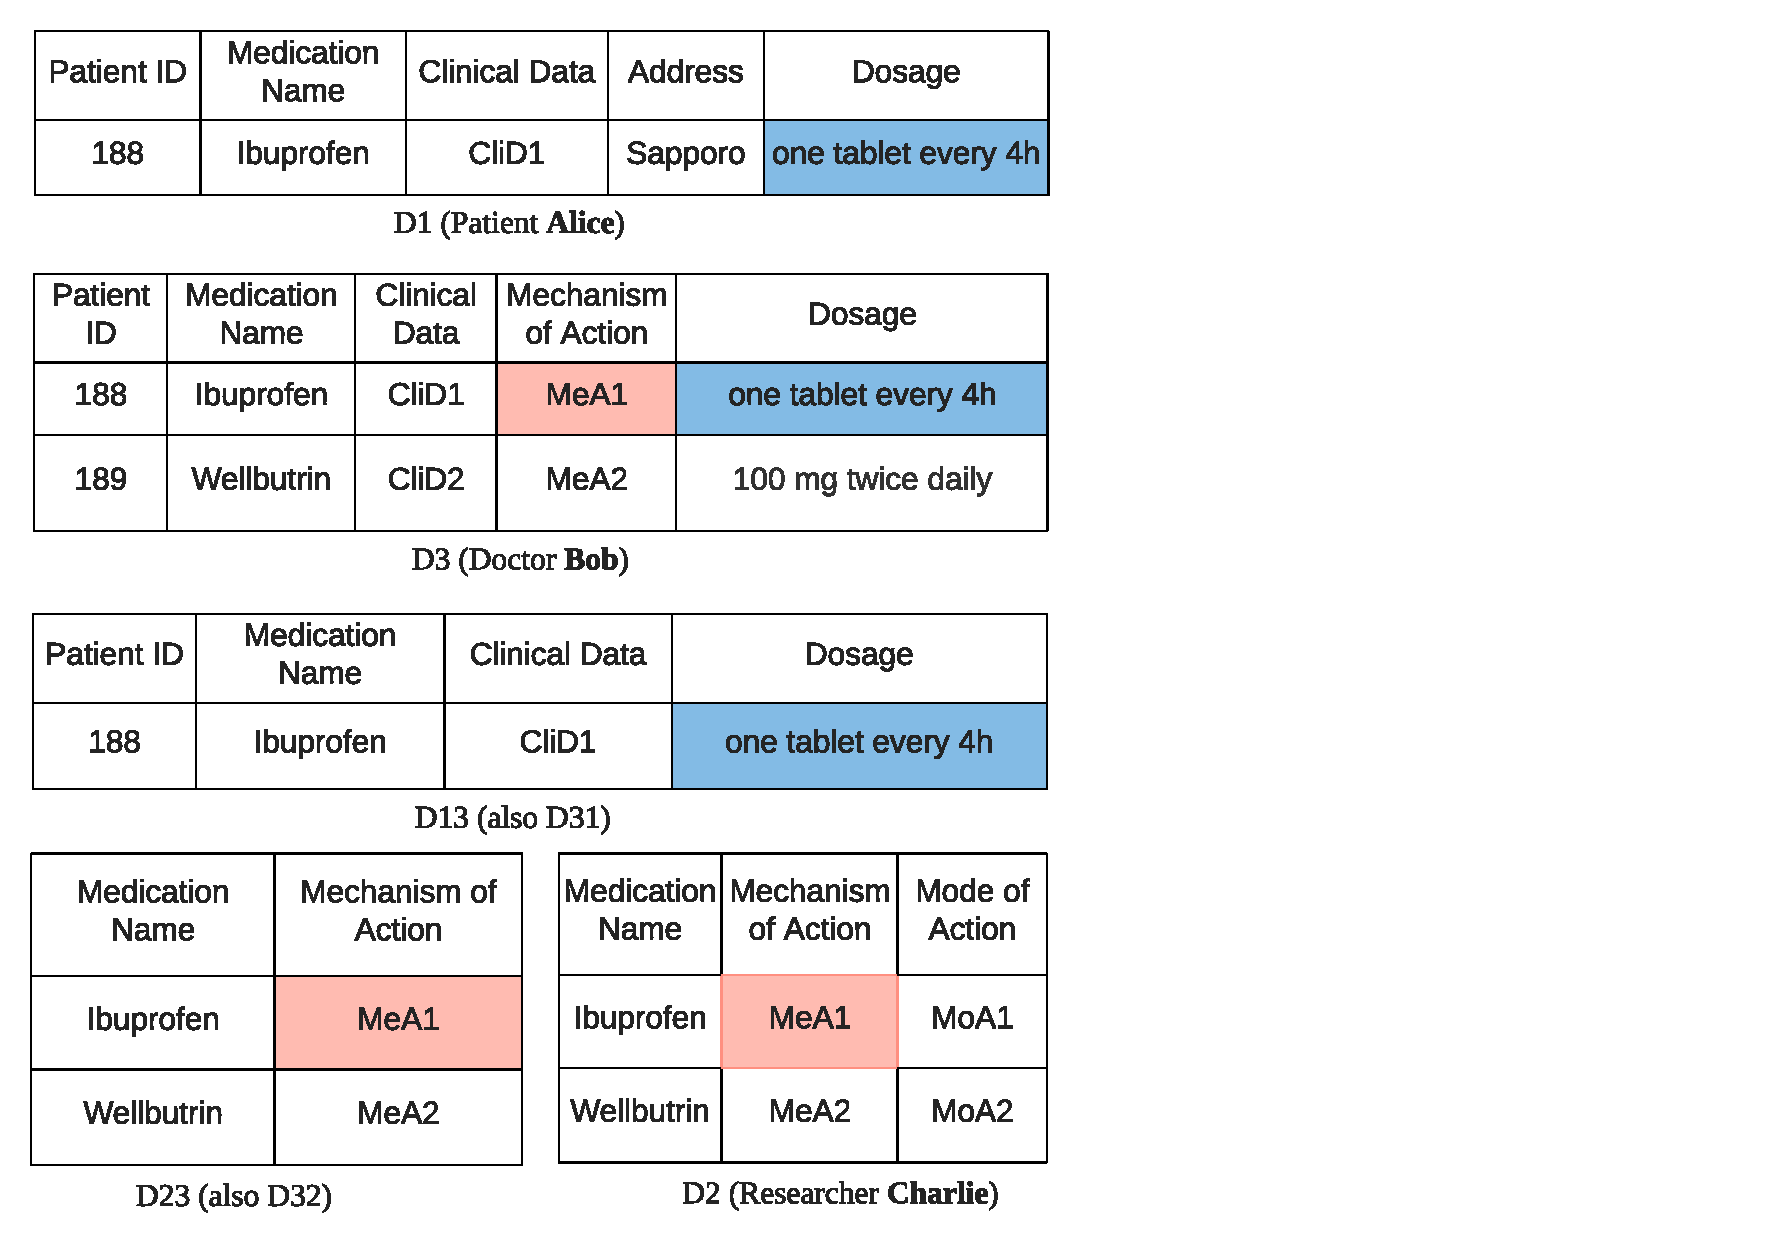
\includegraphics[width=250pt]{medicalData.pdf}}
    \caption{Data distribution}
    \label{dataRepresentation}
\end{figure}

%which means that D13 may have different representations with D32.
Figure \ref{dataRepresentation} presents a concrete example with statistics to illustrate this structure. Each user stores a complete medical record and different shared data pieces on their local database.
%For each table, there are some attributes such as medication name and address on D1.  
As we said before, BX programs are used to synchronize the complete data and shared data. Shared data can be seen as views which can be produced from complete records named as sources. For example, Table D13 is shared by Alice and Bob and can be produced from D1 by \emph{$BX_{13}$-get} (i.e., applying the get direction of the BX program between D1 and D13). If D13 is modified, then D1 need to be updated from original D1 and D13 by using  \emph{$BX_{13}$-put}(i.e., invoking put direction of the BX program between D1 and D13) to ensure that the modified D13 can be regenerated from the updated D1.  

In our design, shared data between any two peers are not exposed to the third party, which can keep data privacy between them to some degree. For example, any operations on D23 or D32 can only be known by Charlie and Bob and Alice have no information about this. However, after the change on D32 are reflected in D3, since D3 has been modified, D31 might need to be regenerated by using \emph{$BX_{31}$-get} on D3.

%\subsection{Case analysis}

%
%Dependency 
%Incremental update
%Dependency graph
%
%Just send them data
%Put online; give them link
%Give data to each person
%
%Advantages of having data Locally not on server: 
%fast/easy to access
%Full control own data; change format
%exposed to others (since public available; sensitive data)
%scalability (multi-access server; slow)

\subsection{Permission on data management}
\label{permission}

\begin{figure}[htbp]
    \centerline{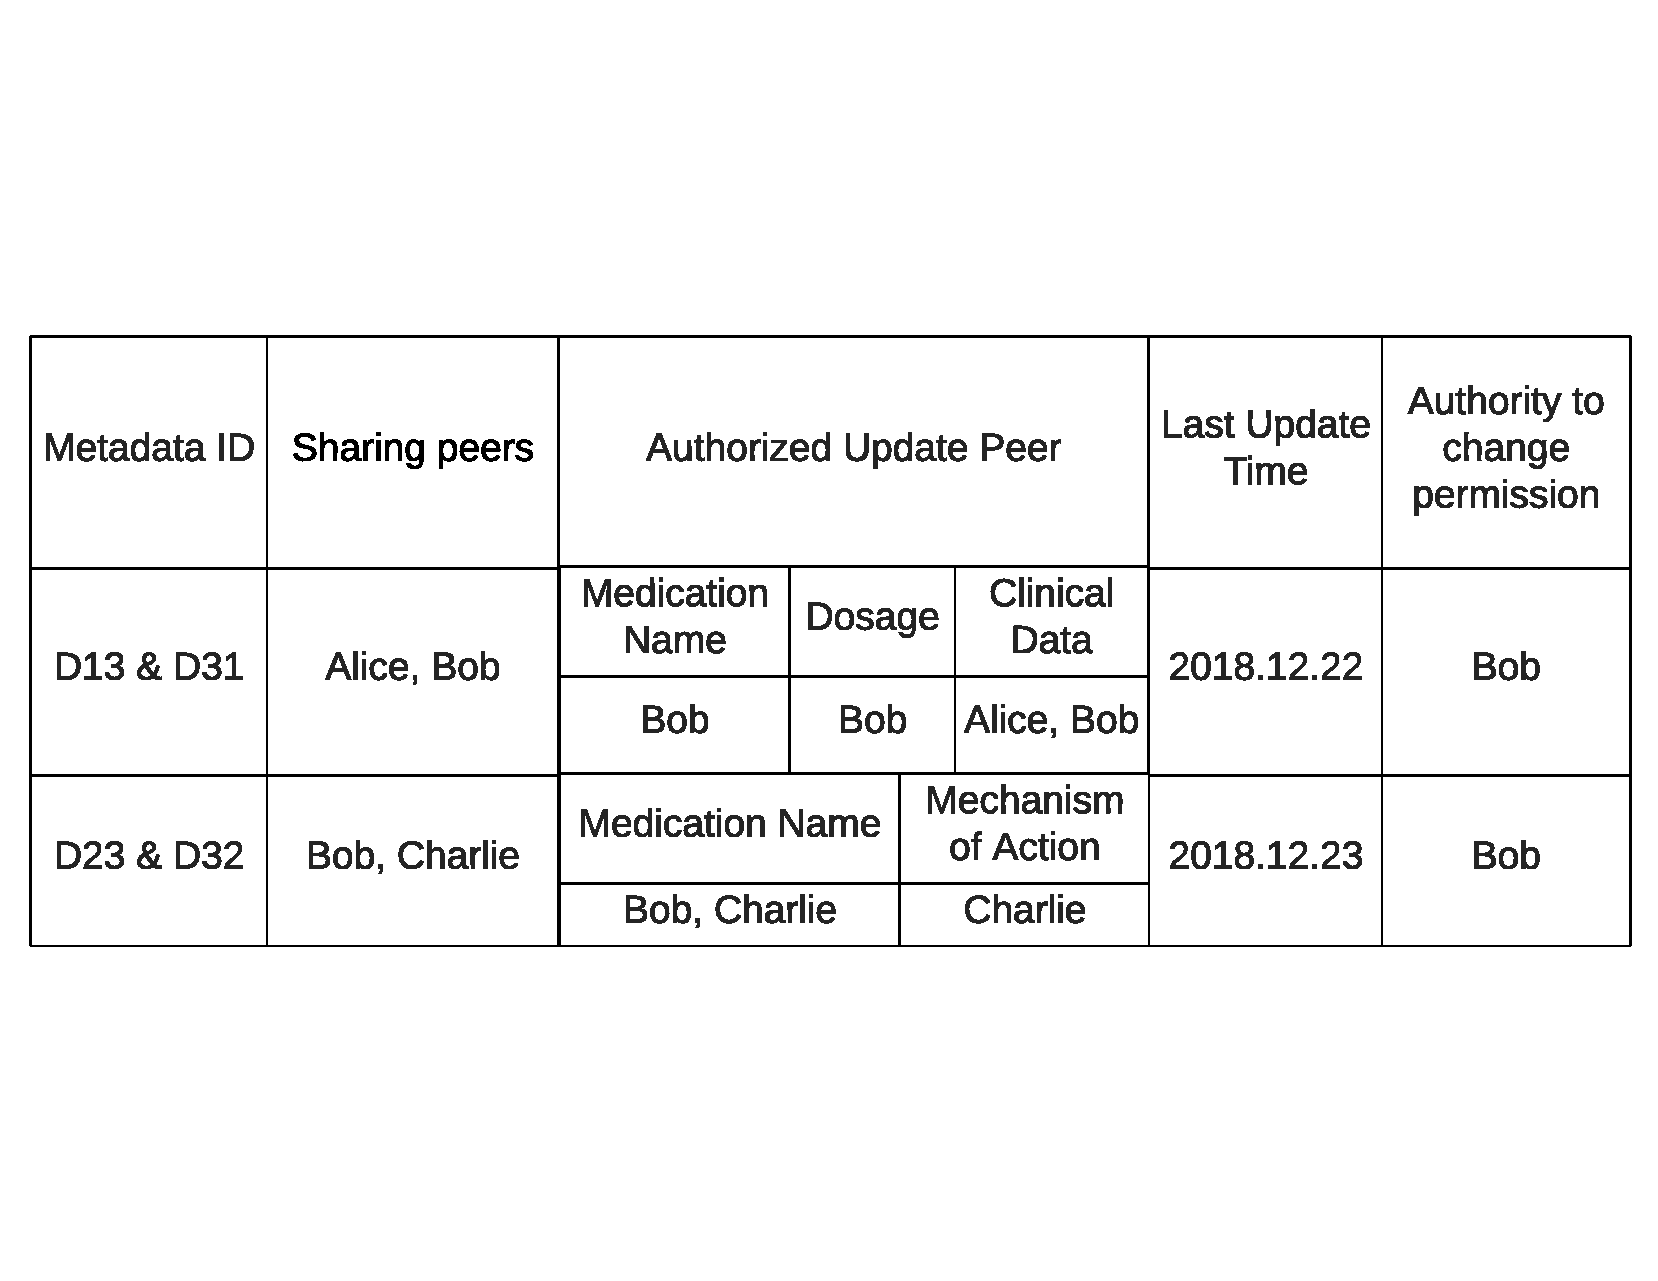
\includegraphics[width=250pt,height=150pt]{metadata.pdf}}
    \caption{Metadata collection in smart contract}
    \label{metadata}
\end{figure}

Figure \ref{metadata} presents a metadata collection table which dictates the update permission on each attribute of the shared data. These kinds of tables reside in smart contracts on the blockchain. Each metadata entry corresponds to a shared table. For example, the entry for D13 or D31 declares that it is shared by Alice and Bob and Bob can update all attributes value but Alice can only change the clinical data. The ``Latest Update Time" shows when the metadata was modified most recently. The value on ``Authority to Change Permission"  delegates Bob to change other peers' (here just Alice) authority. For instance, for D13 and D31, Bob can change the permission to update ``Dosage" to ``Bob, Alice" so that Patient Alice can also update the  ``Dosage" later.

If users want to share data, they need to form an agreement on the structure of the shared table and register the corresponding metadata on smart contracts. Suppose doctor Bob initiates the data sharing with patient Alice. According to their agreement, he will deploy a smart contract on blockchain which stipulates the metadata about the shared data, such as sharing peers (i.e., Alice and Bob) and so on. 

%the ability to modify the update permission are encoded in the field named as ``authority to change permission". 

%Since smart contract cannot be altered after it is deployed on blockchain. 
%
%There are two ways to change the permission for updates to shared data:
%\begin{enumerate}
%    \item deploy a new contract and notify all nodes on blockchain that this new one should be used to control permission;
%    \item update the state of variables in contract.
%\end{enumerate}
%We choose the latter way. In Fig. \ref{dataRepresentation}, 

\subsection{Data Management}
\label{dataManage}

In Fig. \ref{data manage}, we briefly sketch the procedures for CRUD  (i.e., Create, Read, Update, Delete) operations on shared data considering entry level or table level respectively. For Read operation, since shared data just stay in users' local databases, they can just execute a query to get the shared data. Notably, we describe the workflow for updating an item on Section \ref{updateCase}.

\begin{figure}[htbp]
    \centerline{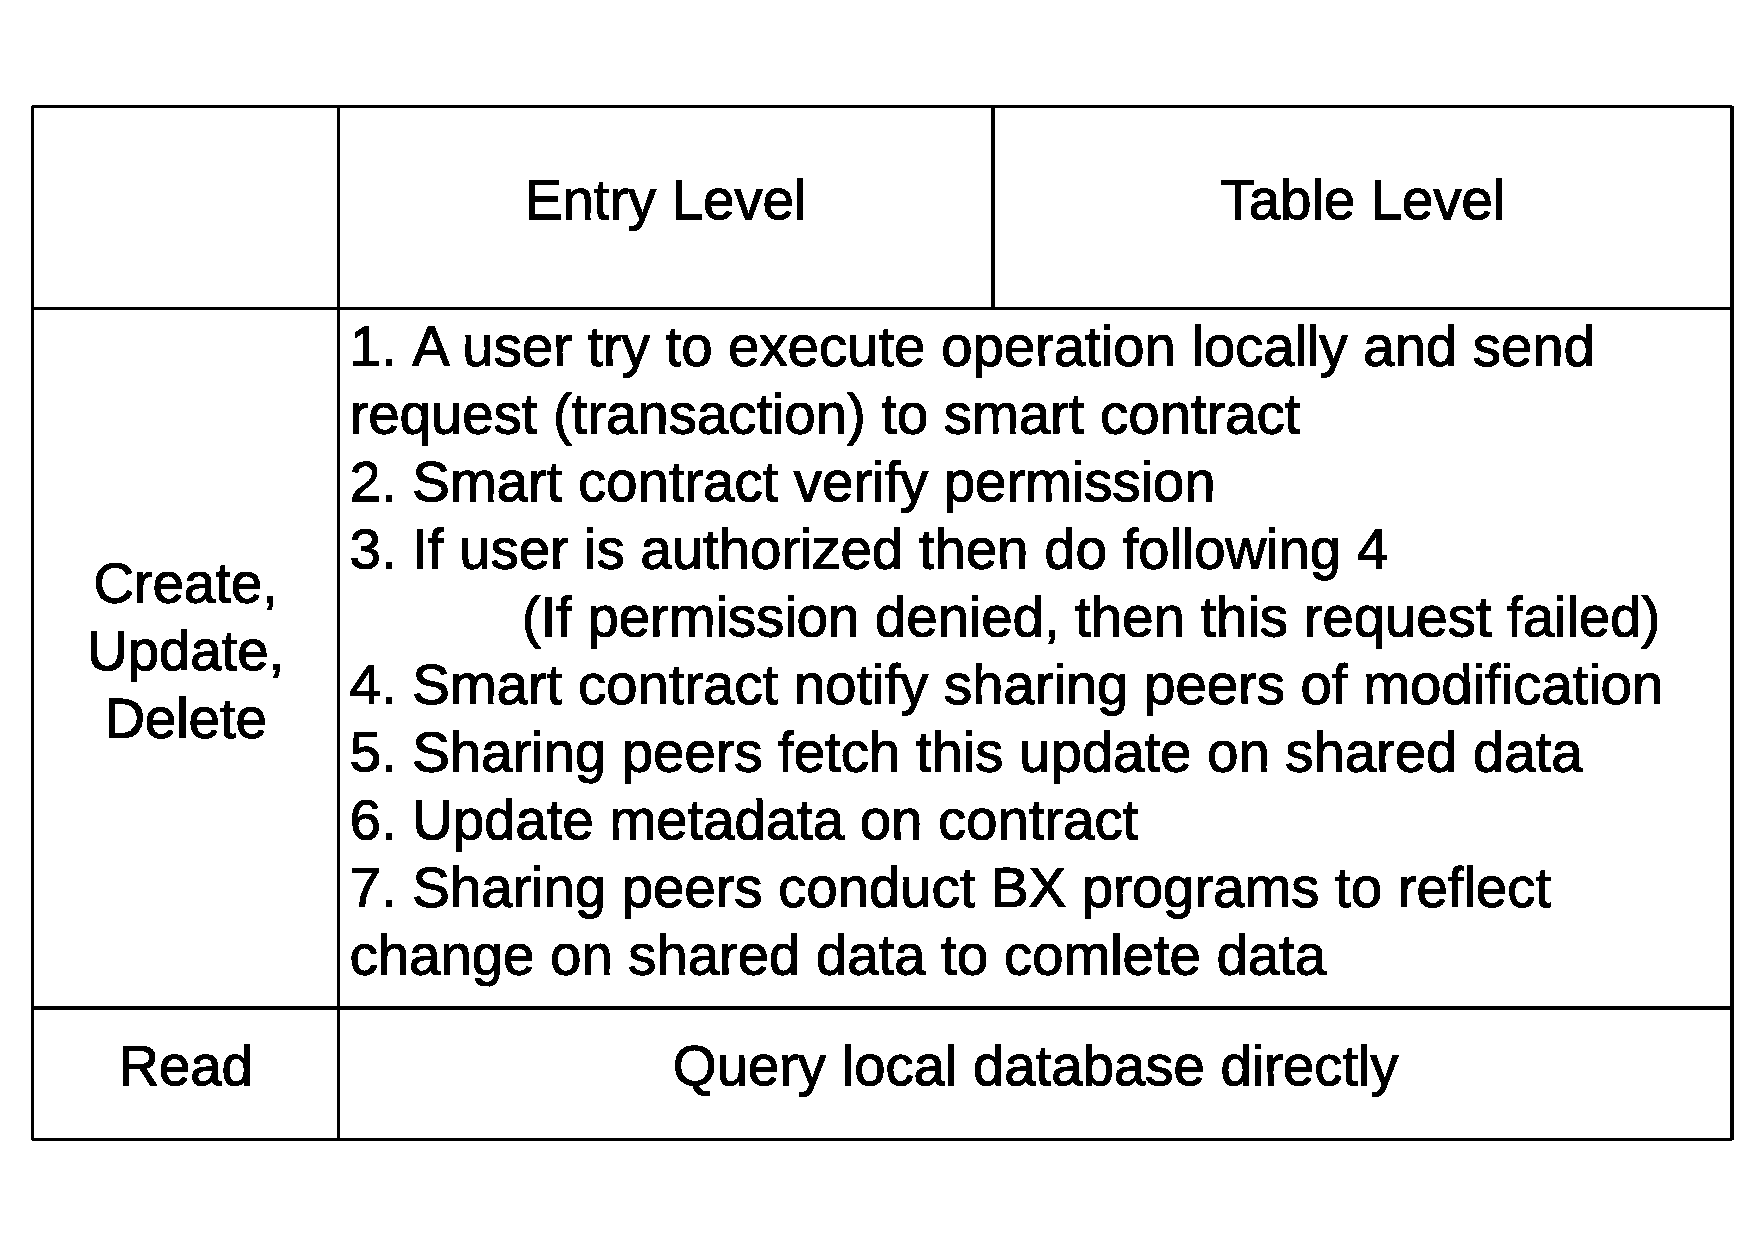
\includegraphics[width=250pt,height=170pt]{dataManage.pdf}}
    \caption{CRUD operations on shared data}
    \label{data manage}
\end{figure}

\subsection{Case analysis for updating shared data}
\label{updateCase}

Figure \ref{workflow} depicts a scenario where the researcher initiates the update the shared data. We use the same notation such as D1 in \ref{fine-grained}. The numbers indicate the corresponding operations sequence. The red and blue circles with wrong sign indicate the updated places. Step 1 - 5 and Step 7 - 11 achieve procedures for an operation on Fig. \ref{data manage}. Notably, step 6 check whether D32 and D31 have some dependencies.  

Let's try to describe this workflow using the data in Fig. \ref{dataRepresentation}. After updating the ``MeA1" on D2, the researcher Charlie wants to propagate the update to the shared data D23 so he uses the \emph{$BX_{23}$-get} to regenerate D23 (step 1). Then he will call a smart contract via a node connected to Ethereum by sending the request for updates to the D23 (step 2). Note that the smart contract in Fig. \ref{metadata}  records all permission info about that D23. 
The smart contract will be executed until all nodes form a consensus on this update request, which means Charlie is permitted to update D23. Each node will conduct the smart contract locally. The entry relating D23 \& D32 of the contract is modified and the doctor Bob will receive notification that D32 need to modified (step 3). Then he will request data from Charlie by sending a message based on some encrypted communication protocol and get the newest shared data to refresh D32 (step 4). After that, Bob will use \emph{$BX_{32}$-put} to reflect the change on D32 in D3, i.e., update the ``MeA1" to a new name. (step 5). Since Bob shared some data (D31) with patient Alice, he needs to check whether D31 need to be reproduced (step 6). (If there is no need to reproduce, step 6 - 11 will not happen.) For example, Bob may want to modify the ``Dosage" on D31. He will use \emph{$BX_{31}$-get} to regenerate D31 (step 7) and request smart contract for permission to update D13 (step 8). Once allowed, Alice will receive a notification about the change on ``Dosage" (D31) (step 9) and ask Bob to send the updated D31. After Alice get the modified D31 (step 10), he will use this to update D1 via \emph{put} (step 11).  

\subsection{System architecture}
\label{architecture}

To achieve our idea, our system will contain four parts, which can be seen from Fig. \ref{systemArchitecture}.

\begin{figure}[htbp]
    \centerline{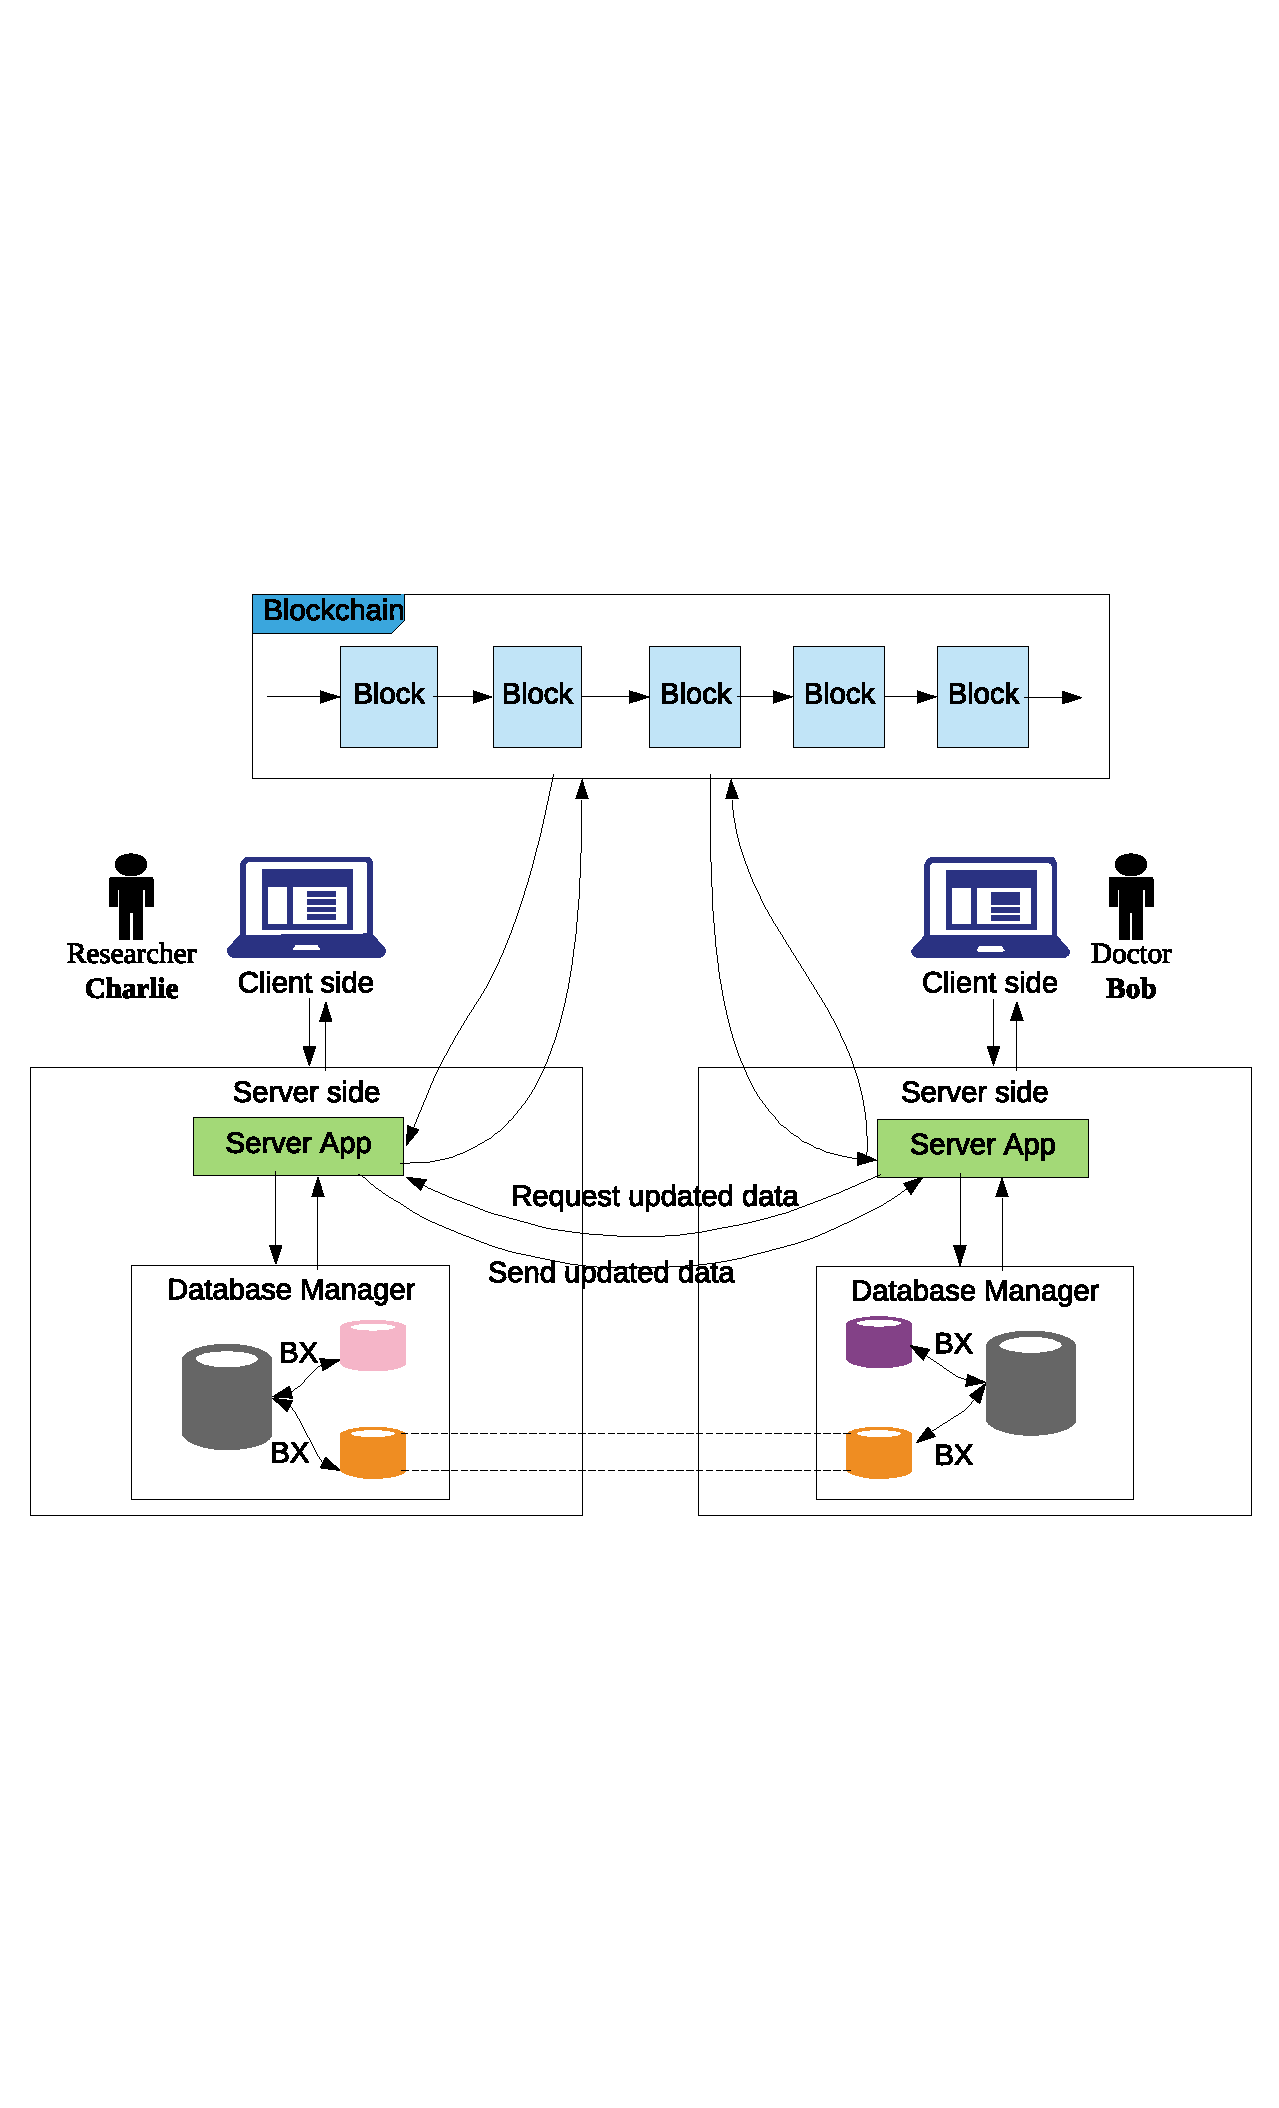
\includegraphics[width=250pt,height=200pt]{systemArchitecture.pdf}}
    \caption{System Architecture}
    \label{systemArchitecture}
\end{figure}

\begin{itemize}
    \item Client side: control the interaction between users and other components.
    
    \item Blockchain: keep the manage permission of shared data on smart contracts and notify sharing peers the change on them.
     
%     Also, front-end user interfaces communicate with blockchain network via nodes. The smart contract on blockchain contains the metadata of shared medical data and maintain a management log that store historical modifications for metadata.
    \item Database manager: disposes of the synchronization between shared data and local data according to consistency logic relations. These synchronizations are implemented by executing BX programs.
    
    \item Database: each user has a complete database and many data pieces shared with other users. The latter (seen as a view) can always be reproduced from the former (seen as a source).
    
\end{itemize}

Next, we discuss more details about this architecture.

% \item nodes can split total data into multiple pieces which can be shared with different nodes, which make sharing exists among only a group of nodes. So that it can avoid the interference or attack from other nodes. 

%    \item Meanwhile, data provider can choose what they want to share with others without exposing sensitive or private information.

%    \item Permission to updates to medical data are stored in smart contracts so that blockchain can prevent operations from malicious nodes. 

Firstly, Raw medical data always stay in each peer's local database and data transfer only exist between sharing peers, which avoid data being leaked to the third party so as to keep shared data security. The data can not only be provided by doctors. Instead, each node can be a shared data provider. As referred in \cite{chung2018using},  many clinics encourage patients to collect data by themselves that are supposed to be gathered by doctors and expect to increase clinic efficiency and promote patient awareness. 

Moreover, blockchain's consensus protocol scheme keep the shared data between sharing peers are same after updates since each peer will receive the notification from contracts and request new shared data from other sharing peers. Additionally, any modification on shared data can be recorded on the blockchain. Blockchain properties such as immutability, auditablility, and transparency enable nodes to check and review update history on shared data. Still, simultaneously updates to the same shared data by multiple peers are forbidden. Smart contracts dispose of the updates according to received requests in chronological order. If a transaction for updates on shared data has been included in a block, then other requests on this shared data will not be accepted, i.e., one block can contain one transaction at most on some shared data at one time. This can promise that only when all sharing peers have had the newest shared data can they execute further operations.

Lastly, this system architecture can also be applied to other data sharing scenarios.

%    \item Any update on shared data can be reflected in local total database by using \emph{put}. Consistency between shared data and local total data are firmly promised by BX. 

\section{Threats and countermeasures}
\label{threats}
 In this section, we identify some threats to our system and propose relating countermeasures.
\subsubsection{Throughput}
We employ smart contracts to control access to shared data. As we all know that the block creation time is approximately 12 seconds on Ethereum. We argue that this time interval is acceptable since nodes may choose to collect a lot of updates then send requests to contracts. Usually, it is not so urgent for a patient or doctor get the immediate updated shared data.

\subsubsection{Correctness of smart contracts }
Smart contracts might be inconsistent with specifications. We may apply some theorem prover such as Coq\cite{huet2004coq} to prove or verify the correctness of smart contracts to prevent these attacks.

\subsubsection{Public blockchain}
Once deployed to the public Ethereum blockchain, transactions relating to our systems might not be chosen into a block by miners. So a private blockchain might be a better choice for our system.

\subsubsection{Incentive}
Like in \cite{dagher2018ancile}, we don't include any incentive for mining beyond the use of our system. We presume that all nodes on the blockchain already have incentives to keep medical data from being tampered and illegal access or updates.

\section{Related work}
\label{related work}
In this section, we review existing blockchain-based research on medical data sharing field and state the advantages of our system compared with them.

Zyskind et al. suggested using blockchain for access control in \cite{zyskind2015decentralizing} where encrypted data reside on the third party storage. But data might be exposed by this ``trusted" the third party so that data privacy is violated.

The idea of introducing Blockchain technology to healthcare was presented firstly in \cite{yue2016healthcare} where they use blockchain for data storage to guarantee medical data cannot be modified by anyone. Also, they designed a Healthcare Data Gateway (HDG) to control access to the shared data. However, the medical data size can become huge so that become a burden for blockchain nodes' storage since each node has the same copy of blockchain. Usually, the size of metadata is smaller than data. (It also depends on the structure of metadata and data.) We store metadata on smart contracts so as to reduce the storage pressure for each blockchain node.
%Similarly, Patientory \cite{mcfarlane2017patientory} proposed that the medical data is stored directly on the HIPPA-compliant blockchain database.  

MedRec \cite{azaria2016medrec} choose to store raw medical data on providers' database and patients can download the data from it after authorized by smart contract on the blockchain. They aimed to enable patients to engage in their healthcare. Whereas in our system, all parties, such as doctors, patients, and researchers can benefit from sharing data with others. MedRec recognized that not all provider data such as physician intellectual property can be exposed to patients \cite{us2017individuals, grossman2011clinical} so that they don't claim to manage contents automatically from physician's output. In our work, instead, we allow each node to share a piece of medical data not total but still keep consistency between them after the updates to the shared ones. Additionally, any modifications on data shared by two nodes will not be disclosed to the third party which keeps the consistency only exists in sharing peers. Moreover, since all shared data with others can be a part of each nodes' local total databases, we can decide whether one shared data have some influence on the other shared pieces and then propagate this change to the third party.

Dubovitskaya at al. gave architecture to manage and share medical data for cancer patient care \cite{dubovitskaya2017secure}. They stored encrypted categorized shared data on the cloud and relating metadata in blockchain and implemented the prototype on Hyperledger\cite{hyperledger2017hyperledger}. The access control policy is defined in the chaincode Logic by patients. Whereas we think that each data provider, not just patients can use smart contracts to encode the control policy when they deploy them to Ethereum. 

Notably, previous three works and others \cite{liu2018bpds,xia2017bbds,amofa2018blockchain,dagher2018ancile,fan2018medblock} mostly targeted to the access problem on shared data but did not pay much attention to updates on them. Additionally, they presumed that different parties can share the same data. Unlike them, we aim to solve the updates issues on the shared data and allow one party can split total data into multiple pieces (i.e, views) which are shared with different parties but still keep consistency between source and views.

%Distributed Authorized Medical Data Management
\section{Conclusion}
\label{conclude}

Medical data sharing are necessary and important, which allow stakeholders on medical scenarios to contribute their knowledge to better the medical treatment. Users may have different interests in the same complete medical record. Some peers might update some values of fields in the existing data. These updates need to be propagated to sharing peers. Our architecture divides a record into pieces that shared with different users separately, which can protect data privacy by limiting essential data between two peers and reduce the unrelated data interference. Any updates on data pieces can be synchronized to complete records by bidirectional transformations. Moreover, based on smart contracts on the blockchain, we can promise that only authorized users can update the existing shared data and only when all peers have updated to the newest data contents they can continue the operations on shared data.   

We are still developing the prototype to implement our idea.
In the future, we will use real patient data to do the experiment but use some de-identification technology to protect patient data from being exposed. 

%\section*{Acknowledgment}
%The authors would like to thank all PRL lab members for their helpful advice in the paper draft.  Thanks Hsiang-Shang Ko for revising the BX parts and providing valuable suggestions to our work. Thanks Van-Dang Tran's help on building the initial data distribution idea sketch. We would like to thank anonymous reviewers for reviewing this paper. This work is partially supported by the Japan Society for the Promotion of Science (JSPS) Grant-in-Aid for Scientific Research (S) No. 17H06099 and Scientific Research (A) No. 18H04093.

\bibliographystyle{IEEEtran}
\bibliography{ref}

\end{document}
